\section{Agent based models}

\begin{frame}{Introduction to Agent-Based Models}
\begin{itemize}

\item \textbf{Definition} Agent-based modeling (ABM) is a methodology used to build formal models of real-world systems that are made up by individual units (such as e.g. people, cells, animals,  or institutions) which repeatedly interact among themselves or with their environment.
    \pause
\item ABM approach establishes a direct a correspondence between the individual units in the system to be modeled and the model the agents and their interactions
\item In other words: Two persons meeting in real world are modeled as meeting of two agents in the model
    \pause
\item This approach contrasts with  equation-based modeling, where modeled system may be represented via average properties.
    \pause
\item Applications: Epidemiology, social sciences, economics, and more.
\end{itemize}
\end{frame}

\begin{frame}{Differences between ABMs and Differential Equation Models}
\begin{itemize}
    \item \textbf{Granularity}: ABMs simulate individual agents, differential equations models represent populations as continuous variables.
    \pause
    \item \textbf{Stochasticity}: ABMs usually include randomness in agents' actions, differential equations models are deterministic (but randomness can be also added).
        \pause
    \item \textbf{Spatial Structure}: ABMs typycally incorporate spatial structures and movement, differential equations models  assume well-mixed populations.
        \pause
    \item \textbf{Complexity}: ABMs handle complex interactions and adaptations, differential equations models focus on average rates of change.
\end{itemize}
\end{frame}

\begin{frame}{Advantages of Agent-Based Models}
\begin{itemize}
    \item \textbf{Emergence}: Emergence occurs when a complex entity has properties or behaviors that its parts do not have on their own, and emerge only when they interact in a wider whole. Think of snow flakes or ant colonies. In ABMs, higher-level system properties may emerge from the interactions of lower-level agents.
        \pause
    \item \textbf{Detail}: Ability to model systems at the level of individual agents allows for detailed exploration of wide range of behavior. 
        \pause
    \item \textbf{Adaptability}: Agents can be programmed to adapt their behaviors in response to changing  conditions or rules.
        \pause
    \item \textbf{Customization}: Models can be easily tailored to specific situations by altering rules, behaviors, and interactions of agents.
\end{itemize}
\end{frame}

\begin{frame}{Disadvantages of Agent-Based Models}
\begin{itemize}
    \item \textbf{Computational Demands}: High complexity and detail level can lead to significant computational costs.
        \pause
    \item \textbf{Data Requirements}: Developing realistic models often requires detailed empirical data, which may not always be available.
        \pause
    \item \textbf{Analysis Complexity}: The richness of the output can make analysis and interpretation challenging.
        \pause
    \item \textbf{Reproducibility Issues}: Due to stochastic elements, reproducing results can be difficult.
        \pause
    \item \textbf{Validation Challenges}: Validating the model against real-world outcomes can be complicated due to the complexity of the models.
\end{itemize}
\end{frame}




\begin{frame}{Applications of Agent-Based Models - Specific Examples}
\only<1>{
\footnotesize
\textbf{Epidemiology}: Modeling the spread of COVID-19 to evaluate the effectiveness of social distancing measures in various communities. Agent-based model \textit{Coves} was developed to help policymakers make decisions based on the best available data, while taking into account the large uncertainties in terms of COVID-19 transmission dynamics, disease progression, and other aspects.
\vfill
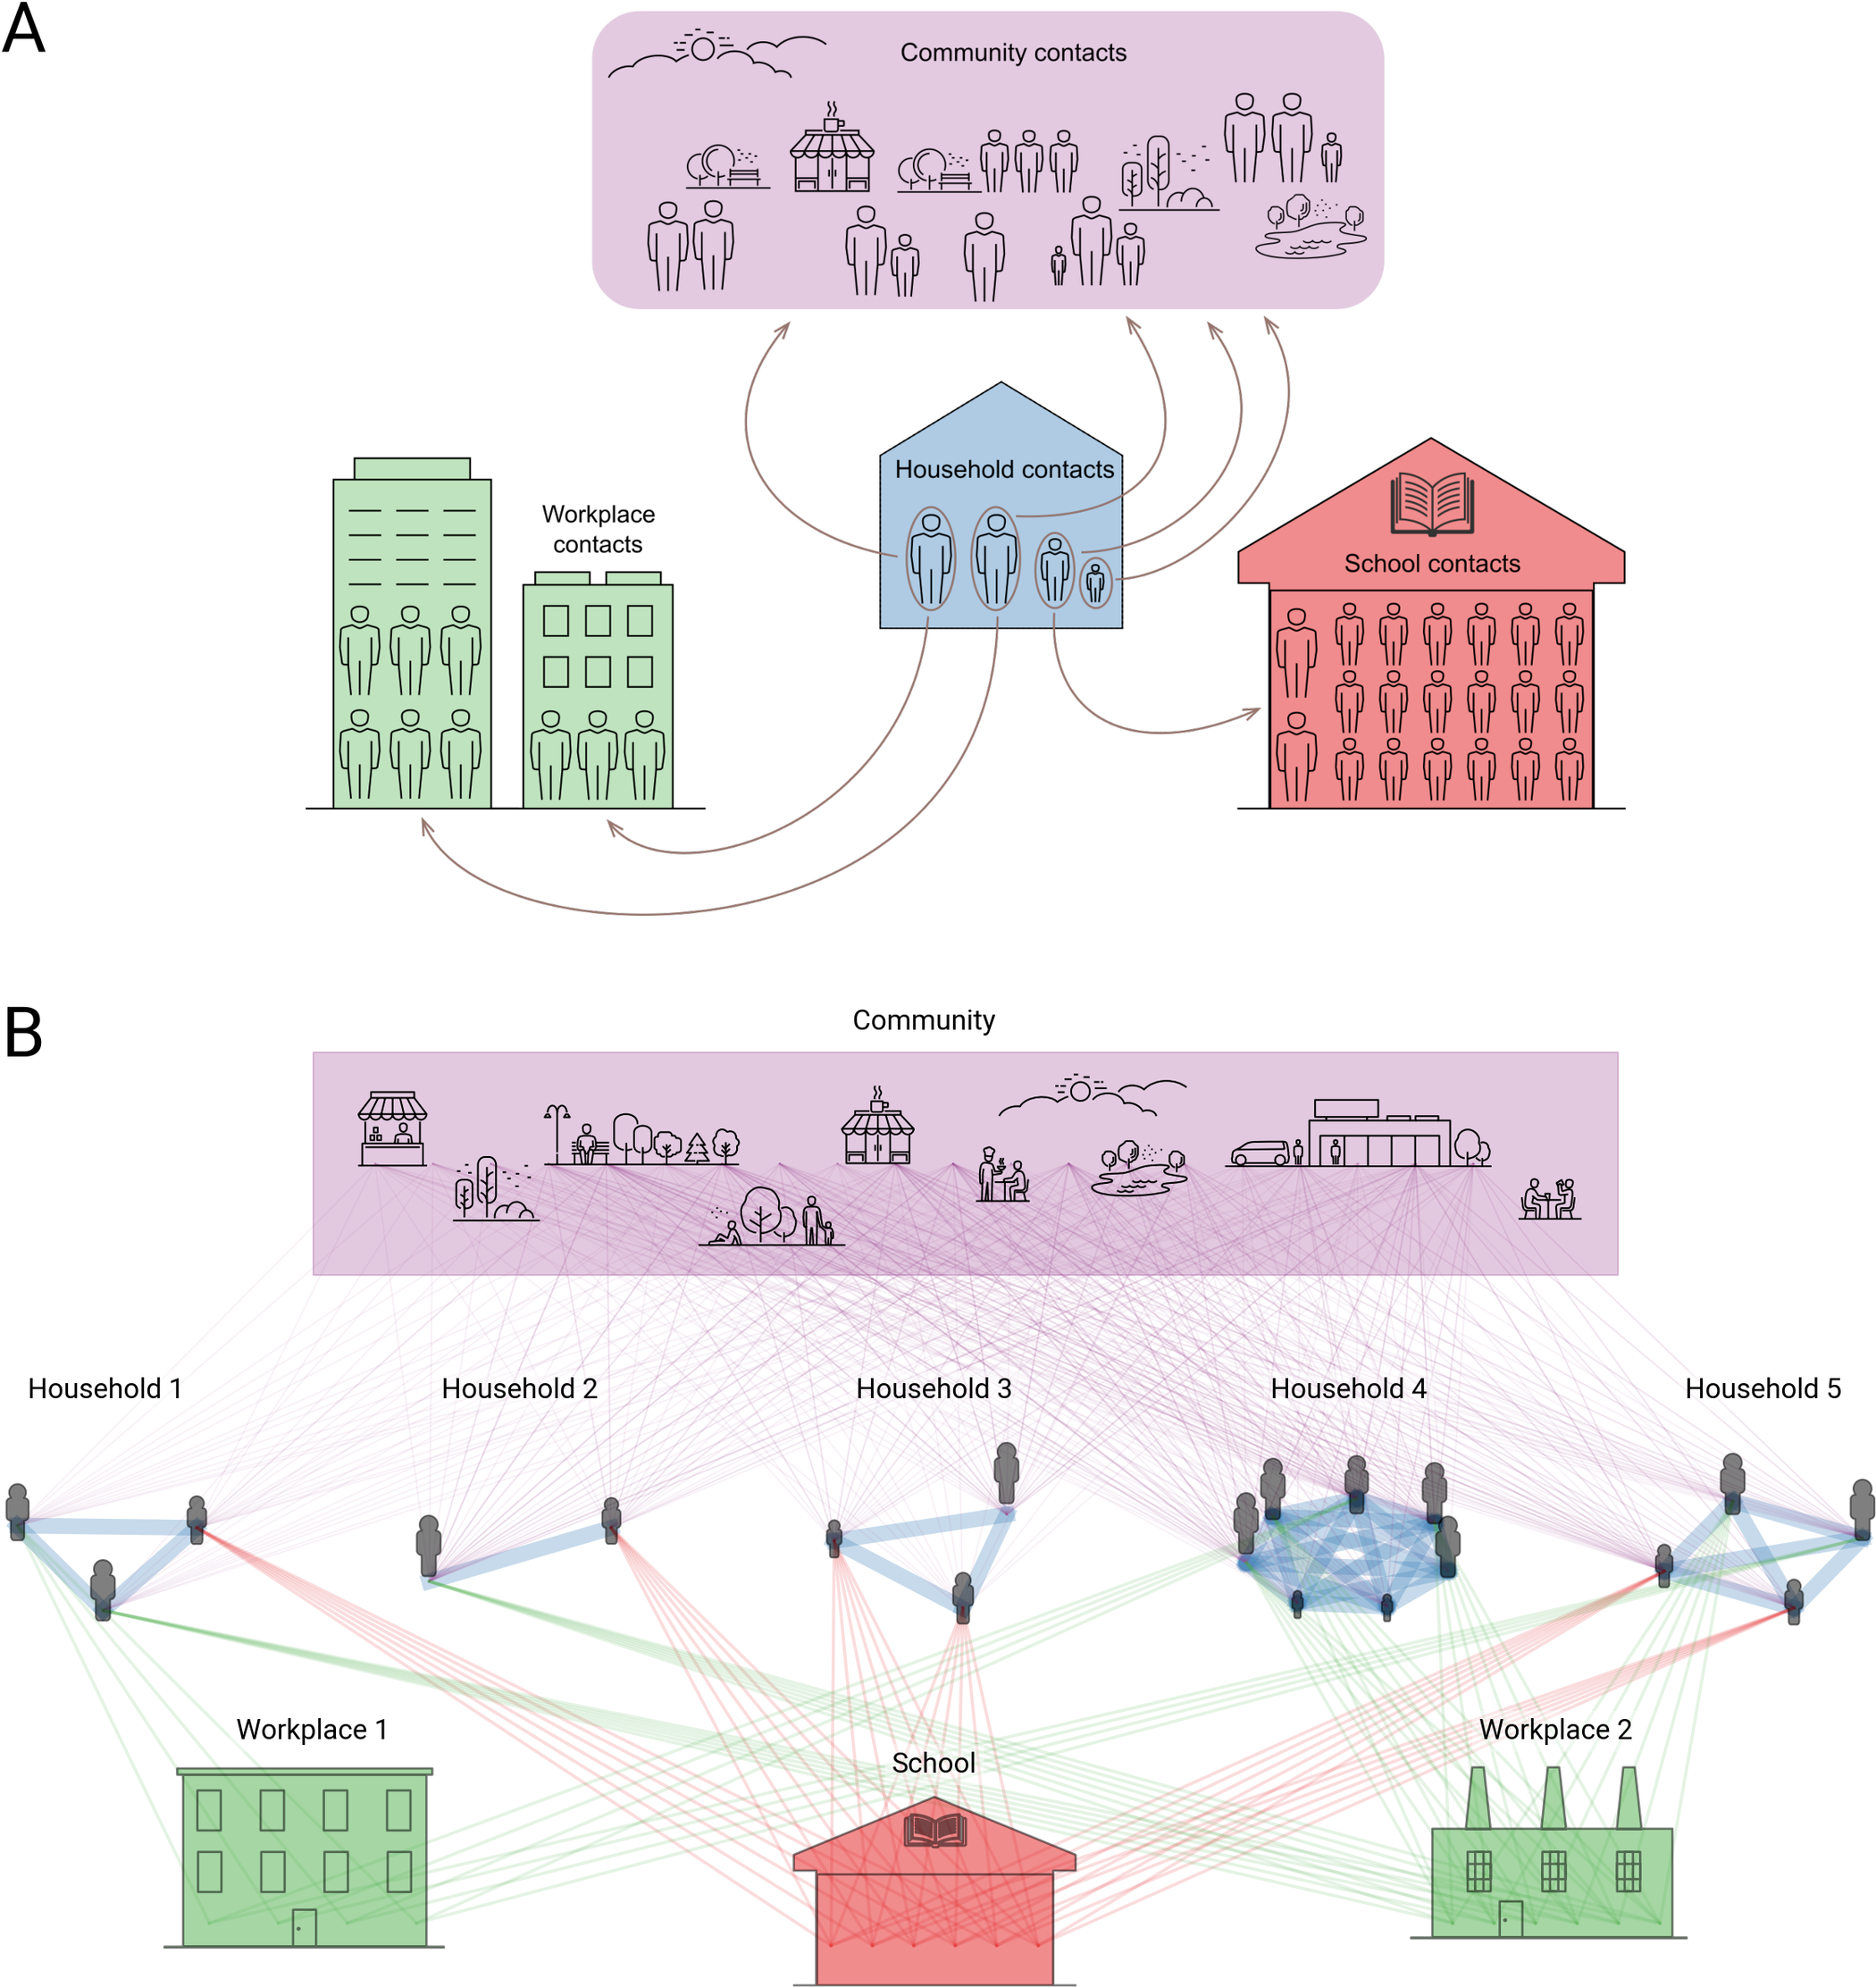
\includegraphics[scale = 0.3]{images/agent_covasim.png}
}
\only<2>{ 
\textbf{Ecology}: Simulation of agent-based model of collective nest choice by the ant. Helps in testing the effects and importance of alternative parameter values and decision rules on colonial decision making.
\vfill 
\textbf{Economics}: Analyzing consumer behavior in online stores to predict reactions to changes in price or product availability. May be used for optimizing pricing strategies.
\vfill 
\textbf{Urban Planning}: Planning public transportation systems by simulating the movement patterns of individuals within a city. Helps in making public transport more efficient and accessible.
\vfill 
\textbf{Social Sciences}: Studying the spread of information and misinformation through social networks to understand the dynamics of public opinion formation. 
\vfill
\textbf{Military}: An agent-based computational model for the Battle of Trafalgar. Help to decide what outcomes were possible or what environmental factors has affected the results. 
}
\end{frame}


\begin{frame}{Basics of an Agent-Based SIR Model}
\begin{itemize}
    \item \textbf{Agents}: Represent individuals in a population, each with a position on a 2-D grid.
    \item \textbf{States}: Susceptible, Infected, Recovered.
    \pause
    \item \textbf{Rules of Transition}:
    \begin{itemize}
        \item Susceptible $\to$ Infected: Probability depends on \textbf{distance} to nearby infected agents and decays with range.
        \item Infected $\to$ Recovered: Each step with probability $p_{\text{recover}}$.
    \end{itemize}
        \pause
    \item \textbf{Movement}: Each agent performs a random walk (one step per tick) on a bounded grid.
    \item \textbf{Simulation}: Iterative loop updating health states and positions until a set number of steps is reached.
\end{itemize}
\end{frame}


\begin{frame}{Agent Movement: Random Walk}
  \begin{center}
    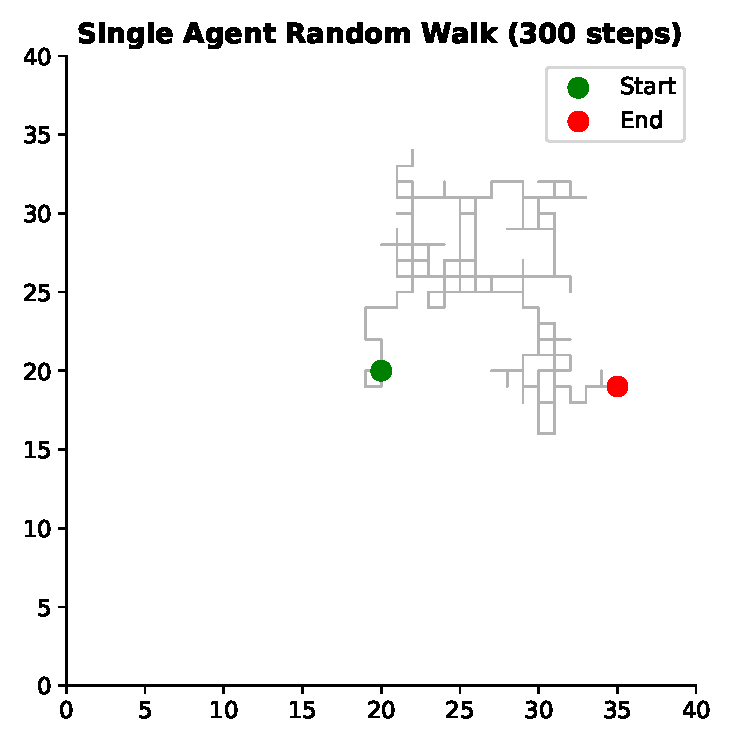
\includegraphics[width=0.5\textwidth]{images/abm_random_walk.pdf}
  \end{center}
  \small
  Each agent performs a discrete random walk on a bounded grid. At every step the agent moves one cell in a random cardinal direction. Boundary cells reflect the agent back inward.
\end{frame}

\begin{frame}{Advantages of ABMs in Epidemic Modeling}
\begin{itemize}
    \item \textbf{Flexibility}: Can model complex behaviors and interventions (e.g., social distancing, quarantine).
        \pause
    \item \textbf{Heterogeneity}: May account for individual differences in susceptibility, immunity and mobility.
        \pause
    \item \textbf{Spatial Dynamics}: Models how the disease spreads in physical space, including community structures.
        \pause
    \item \textbf{Data Integration}: Can incorporate empirical data at the individual level to calibrate or validate the model.
\end{itemize}



\end{frame}


\begin{frame}{Distance-Based Transmission Model}
\small
Instead of requiring agents to share the exact same cell, we use a \textbf{distance-dependent} infection probability.
\pause
\vfill
Each infected agent within radius $r_{\text{infect}}$ poses an independent risk. The contribution from one infected neighbour at distance $d$ is:
\[
  p_i = p_{\text{infect}} \cdot e^{-d\, /\, r_{\text{infect}}}
\]
\pause
When multiple infected agents are nearby, the combined probability is:
\[
  P = 1 - \prod_{i}(1 - p_i)
\]
\vfill
\begin{block}{Two real-world effects captured}
\begin{itemize}
  \item \textbf{Distance matters} --- close contacts are far more dangerous than distant ones.
  \item \textbf{Multiple exposures compound} --- being surrounded by several infected agents is much riskier.
\end{itemize}
\end{block}
\end{frame}

\begin{frame}{Transmission Probability vs.\ Distance}
  \begin{center}
    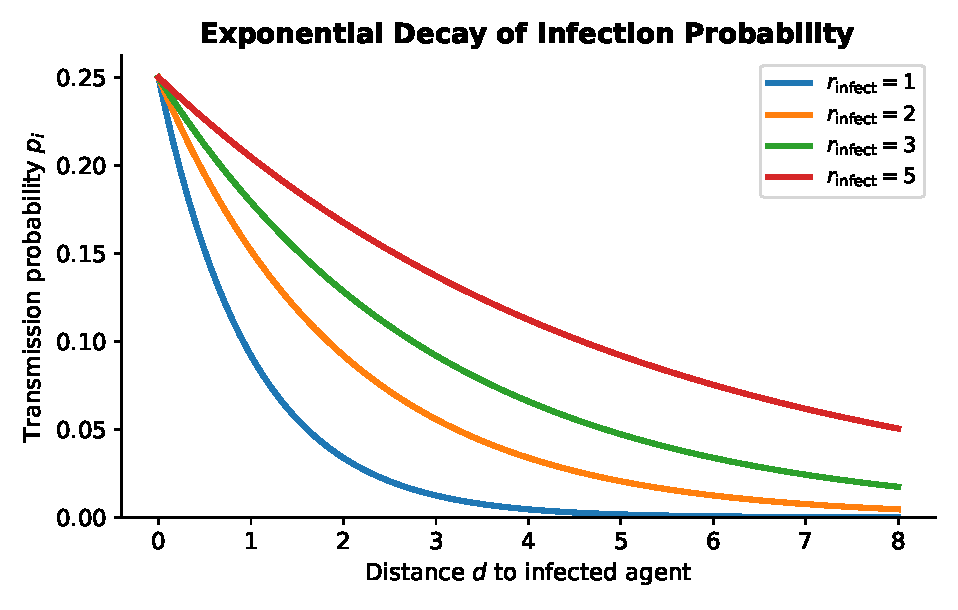
\includegraphics[width=0.85\textwidth]{images/abm_transmission_decay.pdf}
  \end{center}
  \small
  The base probability $p_{\text{infect}} = 0.25$ decays exponentially. A larger infection radius means the probability remains significant over longer distances.
\end{frame}

\begin{frame}{Compounding Risk from Multiple Neighbours}
  \begin{center}
    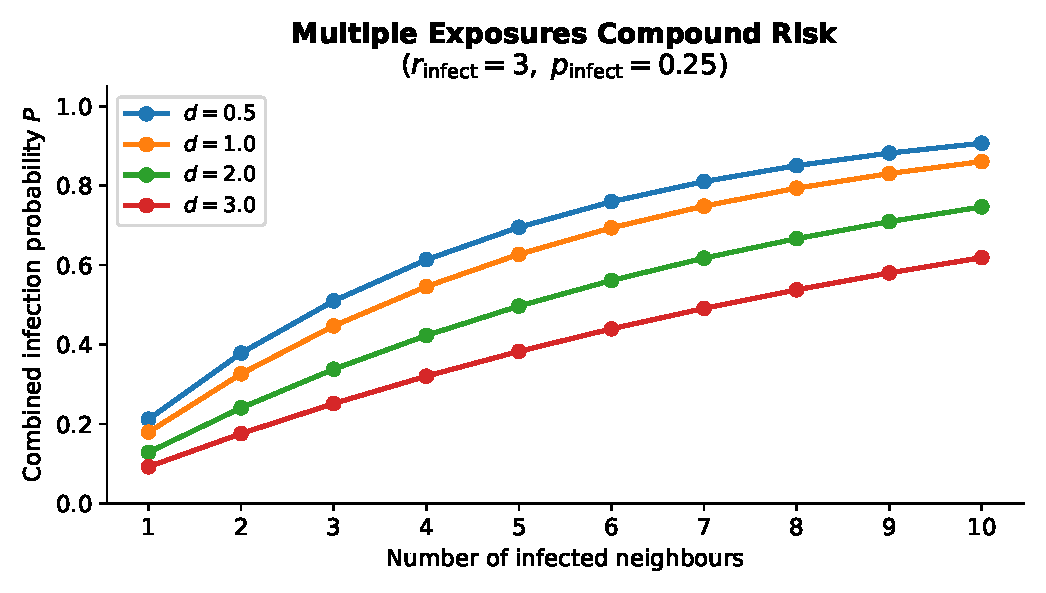
\includegraphics[width=0.85\textwidth]{images/abm_compound_probability.pdf}
  \end{center}
  \small
  Even if each individual contact carries moderate risk, the combined probability grows quickly with the number of infected neighbours --- especially at close range.
\end{frame}

\begin{frame}{Simulation Loop in an Agentic SIR Model}
\footnotesize
\begin{itemize}

    \item \textbf{Update States:}
    \begin{itemize}
    \footnotesize
        \item For each susceptible agent, compute the combined infection probability from all infected agents within radius $r_{\text{infect}}$.
        \item Use a random draw against this probability to transition from susceptible to infected.
        \item For each infected agent, use a random draw with the recovery probability to transition to recovered.
    \end{itemize}
    \item \textbf{Record Results:}
    \begin{itemize}
    \footnotesize
        \item Count the number of susceptible, infected, and recovered individuals and store these counts for visualization.
    \end{itemize}
    \item \textbf{Visualization:}
    \begin{itemize}
    \footnotesize
        \item Update  plots showing current positions and a time-series plot tracking S, I, and R dynamics.
    \end{itemize}
    \item \textbf{Update Positions:}
    \begin{itemize}
    \footnotesize
        \item Move each agent using a predefined random movement rule.
        \item Ensure that new positions remain within the simulation boundaries.
    \end{itemize}
\end{itemize}
\end{frame}

\begin{frame}{Effect of Infection Radius}
  \begin{center}
    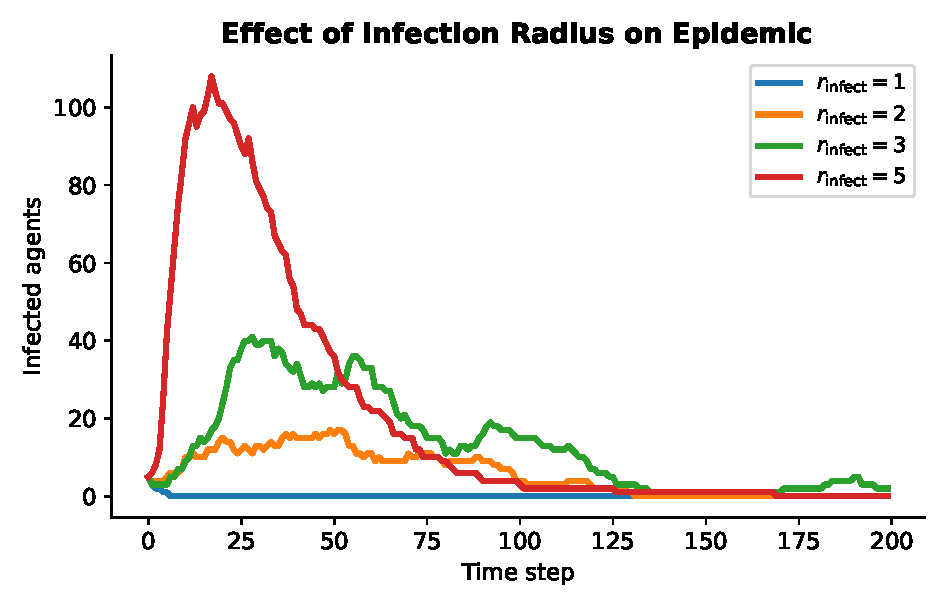
\includegraphics[width=0.85\textwidth]{images/abm_infection_radius.pdf}
  \end{center}
  \small
  Larger $r_{\text{infect}}$ dramatically accelerates the epidemic. A very small radius ($\approx 1$) approximates the original same-cell model where outbreaks spread slowly.
\end{frame}

\begin{frame}{Spatial Snapshots Over Time}
  \begin{center}
    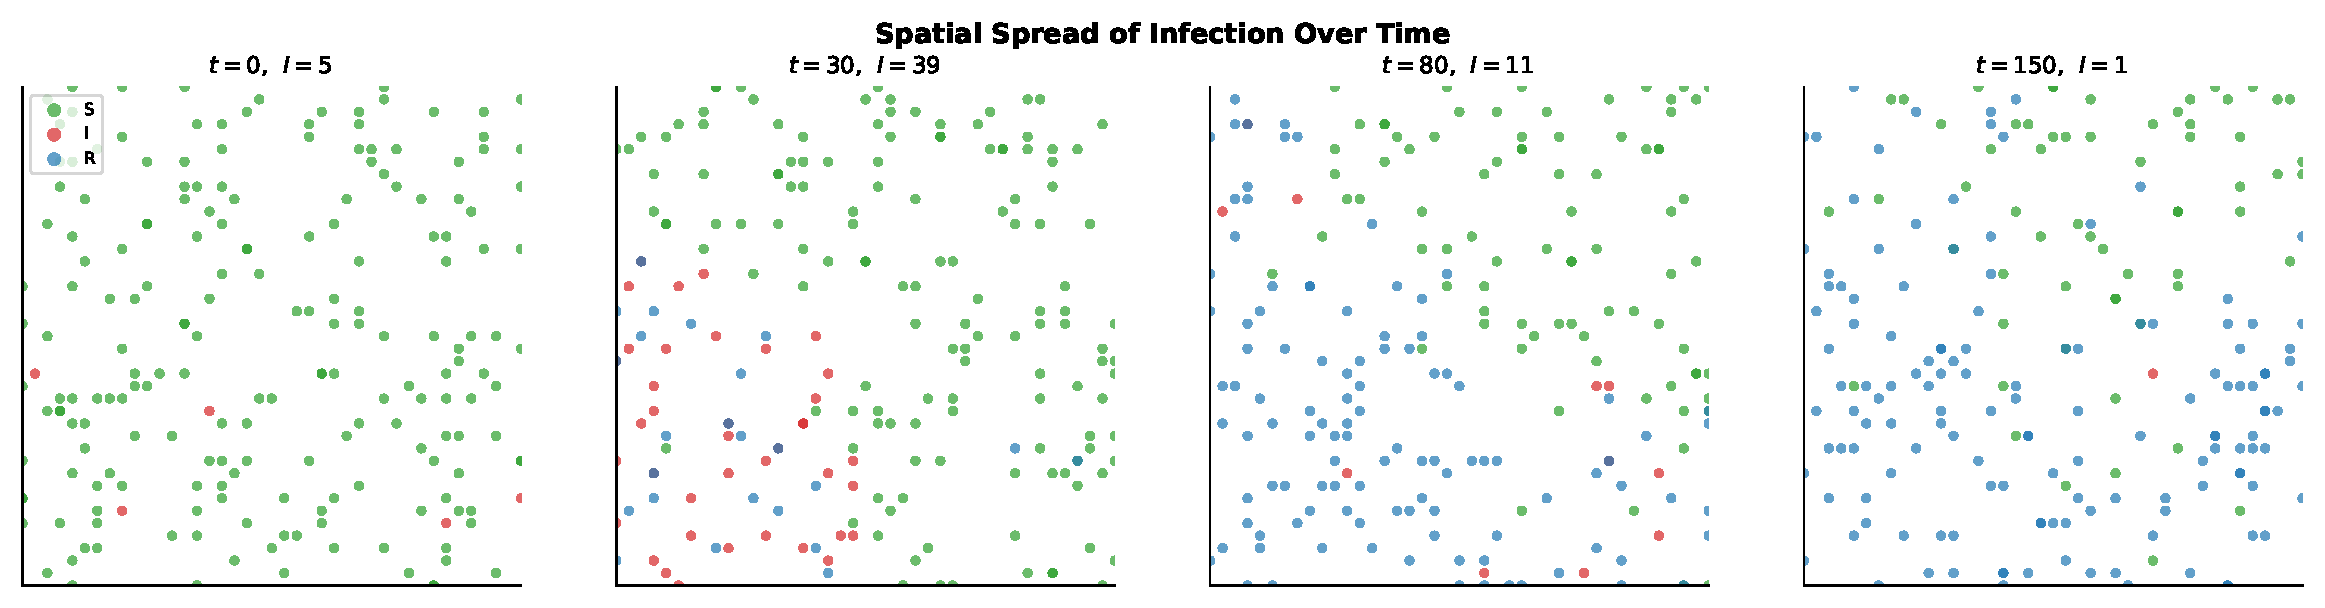
\includegraphics[width=\textwidth]{images/abm_spatial_snapshots.pdf}
  \end{center}
  \small
  Infection clusters form around the initial cases, expand as agents wander, and leave a growing ``barrier'' of recovered (blue) agents.
\end{frame}

\begin{frame}{Visualising Epidemic Dynamics}
  \begin{itemize}
    \item \textbf{Epidemic curves}: Time-series plots of S, I, R counts reveal peak timing and outbreak size.
    \pause
    \item \textbf{Spatial snapshots}: Scatter plots at selected time steps show how infection clusters form, grow, and merge.
    \pause
    \item \textbf{Animation}: A frame-by-frame animation of agent positions coloured by state provides the most complete picture of spatial dynamics.
    \begin{itemize}
      \footnotesize
      \item Reveals how agents wander, how infection fronts propagate, and how the recovered ``barrier'' gradually forms.
      \item Built with \texttt{matplotlib.animation.FuncAnimation} and rendered inline in Jupyter.
    \end{itemize}
    \pause
    \item \textbf{Parameter exploration}: Varying $p_{\text{infect}}$, $p_{\text{recover}}$, and $r_{\text{infect}}$ shows how each parameter shapes the epidemic.
  \end{itemize}
\end{frame}
